\section{Experiment configurations}
\label{app:configs}
Every row below corresponds to a run in \texttt{reports/experiment\_log.jsonl} and a TensorBoard directory \texttt{logs/tensorboard/<run ID>}. All runs used the same stratified 70/15/15 split (seed 42). Traditional models used median imputation with missing-value indicators, 0.1/99.9\% winsorising of continuous variables and one-hot encoded smoking status; logistic regression (except E02) and all networks were also standardised. Run IDs are from the final reported execution.

\begin{footnotesize}
\begin{longtable}{@{}p{0.04\linewidth}p{0.17\linewidth}p{0.41\linewidth}p{0.32\linewidth}@{}}
\toprule
ID & Run ID & Hyper-parameters & Observation (after reading the results)\\
\midrule
\endhead
E01 & \texttt{E01\_20261018T073349Z} & C=1.0, penalty=l2, solver=lbfgs, max\_iter=1000 & Reference model: converges in 36 iterations; 0.86 accuracy hides 0 prediabetes and 0.18 diabetes recall under argmax. \\
E02 & \texttt{E02\_20261018T073416Z} & C=1.0, penalty=l2, solver=lbfgs, max\_iter=200, scaling=False & Without scaling, L-BFGS hits its 200-iteration cap (convergence warning), runs ~5x slower and is worse than E01 on every metric. \\
E03 & \texttt{E03\_20261018T073421Z} & C=1.0, penalty=l2, solver=lbfgs, max\_iter=1000 & Balanced weights vs E01: diabetes recall 0.18->0.59, prediabetes 0->0.31, but accuracy 0.645 and macro AP drops slightly; threshold moved, ranking not improved. \\
E04 & \texttt{E04\_20261018T073449Z} & n\_estimators=150, max\_depth=None, min\_samples\_leaf=5, max\_features=sqrt & Fully grown trees (mean depth ~39, ~13k leaves): macro AP above E01 but ROC-AUC below it, the signature of a high-variance learner. \\
E05 & \texttt{E05\_20261018T073517Z} & learning\_rate=0.1, max\_iter=200, max\_leaf\_nodes=31, min\_samples\_leaf=20 & Boosting improves both macro AP and ROC-AUC over the forest: sequential bias reduction beats averaging deep trees here. \\
E06 & \texttt{E06\_20261018T073551Z} & learning\_rate=0.1, max\_iter=200, max\_leaf\_nodes=31, min\_samples\_leaf=20 & Engineered features add only +0.0004 macro AP to E05; trees already form interactions such as age x BMI by splitting. \\
E07 & \texttt{E07\_20261018T075447Z} & l2\_regularization=4.33792, learning\_rate=0.03629, max\_iter=587, max\_leaf\_nodes=16, min\_samples\_leaf=73 & Search picks the most regularised candidate (lr 0.036, 16 leaves, L2 4.34; train-fold 0.625 vs CV 0.475): best macro AP of all runs. \\
E08 & \texttt{E08\_20261018T075614Z} & l2\_regularization=4.33792, learning\_rate=0.03629, max\_iter=587, max\_leaf\_nodes=16, min\_samples\_leaf=73 & Balanced weights on E07 repeat the E03 pattern: diabetes recall 0.66, prediabetes 0.28, macro AP lower. \\
E09 & \texttt{E09\_20261018T080006Z} & max\_depth=14, max\_features=0.1572, min\_samples\_leaf=6, n\_estimators=300 & Shallower forest (depth 14, ~16\% features per split) raises ROC-AUC 0.786->0.792 at unchanged macro AP: regularisation smooths mid-risk ranking. \\
E10 & \texttt{E10\_20261018T080040Z} & layers=32, activation=relu, learning\_rate=0.001, dropout=0, l2=0, batch\_size=512, epochs\_run=15, best\_epoch=9, params=1763, optimizer=Adam, early\_stopping=val\_loss, patience 6 & 32-unit MLP early-stops at epoch 9 with a negligible train/val gap; beats LR slightly but trails boosting. \\
E11 & \texttt{E11\_20261018T080233Z} & layers=128-64-32, batch\_norm=True, dropout=0.3, l2=0.0001, learning\_rate=0.001, batch\_size=512, epochs\_run=29, best\_epoch=23, params=17987, optimizer=Adam, early\_stopping=val\_loss, patience 6 & Deeper MLP with BN/dropout/L2: small gain over E10; training loss above validation loss because regularisation is active only in training. \\
E12 & \texttt{E12\_20261018T080307Z} & layers=128-64-32, batch\_norm=True, dropout=0.3, l2=0.0001, learning\_rate=0.01, batch\_size=512, epochs\_run=8, best\_epoch=2, params=17987, optimizer=Adam, early\_stopping=val\_loss, patience 6 & lr 1e-2 is unstable (best epoch 2, oscillating validation loss) and loses macro AP versus E11. \\
E13 & \texttt{E13\_20261018T080645Z} & layers=128-64-32, batch\_norm=True, dropout=0.3, l2=0.0001, learning\_rate=0.0001, batch\_size=512, epochs\_run=60, best\_epoch=60, params=17987, optimizer=Adam, early\_stopping=val\_loss, patience 6 & lr 1e-4 is still improving at the 60-epoch cap and takes ~2x E11's time for the same macro AP: too slow for the budget. \\
E14 & \texttt{E14\_20261018T080856Z} & layers=128-64-32, batch\_norm=True, dropout=0.3, l2=0.0001, learning\_rate=0.001, batch\_size=4096, epochs\_run=60, best\_epoch=58, params=17987, optimizer=Adam, early\_stopping=val\_loss, patience 6 & Batch 4096 needs 58 of 60 epochs to match E11: fewer updates per epoch, no quality gain. \\
E15 & \texttt{E15\_20261018T081015Z} & layers=128-64-32, batch\_norm=True, dropout=0.3, l2=0.0001, learning\_rate=0.001, batch\_size=512, epochs\_run=19, best\_epoch=13, params=17987, optimizer=Adam, early\_stopping=val\_loss, patience 6 & Softened class weights raise diabetes recall 0.16->0.50 and macro-F1 to 0.454 with macro AP unchanged; prediabetes still never predicted. \\
E16 & \texttt{E16\_20261018T081202Z} & architecture=wide (linear) + deep 128-64, logits summed, dropout=0.3, l2=0.0001, learning\_rate=0.001, batch\_size=512, epochs\_run=29, best\_epoch=23, params=16031, optimizer=Adam, early\_stopping=val\_loss, patience 6 & Wide-and-deep is the best deep model: the linear wide path keeps the additive signal, the deep path adds little on top. \\
E17 & \texttt{E17\_20261018T081347Z} & architecture=wide (linear) + deep 128-64, logits summed, dropout=0.3, l2=0.0001, learning\_rate=0.001, batch\_size=512, epochs\_run=29, best\_epoch=23, params=17603, optimizer=Adam, early\_stopping=val\_loss, patience 6 & Engineered features give no gain on E16, consistent with E06. \\
\bottomrule
\end{longtable}
\end{footnotesize}


\section{Supplementary figures}

\begin{figure}[H]
\centering
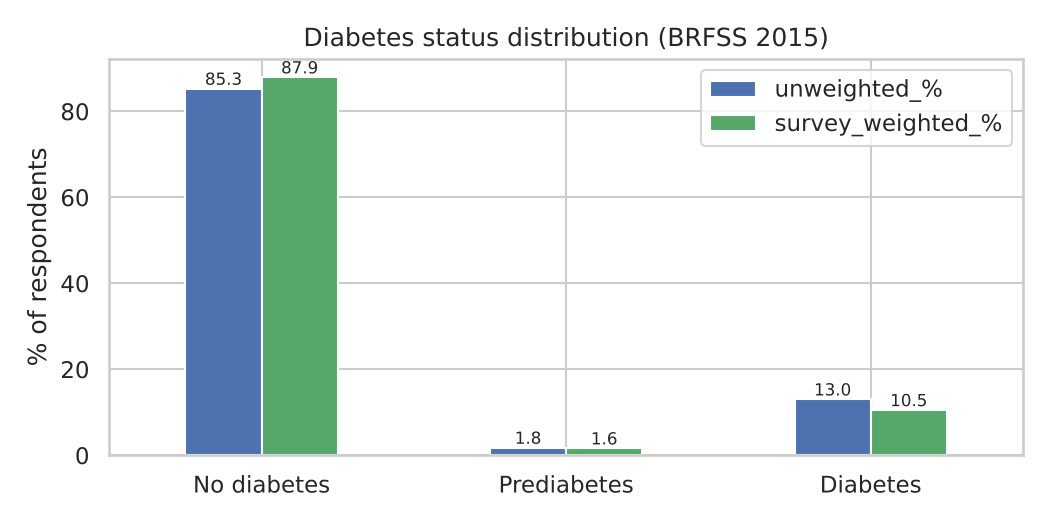
\includegraphics[width=0.48\linewidth]{fig01_target_distribution.png}\hfill
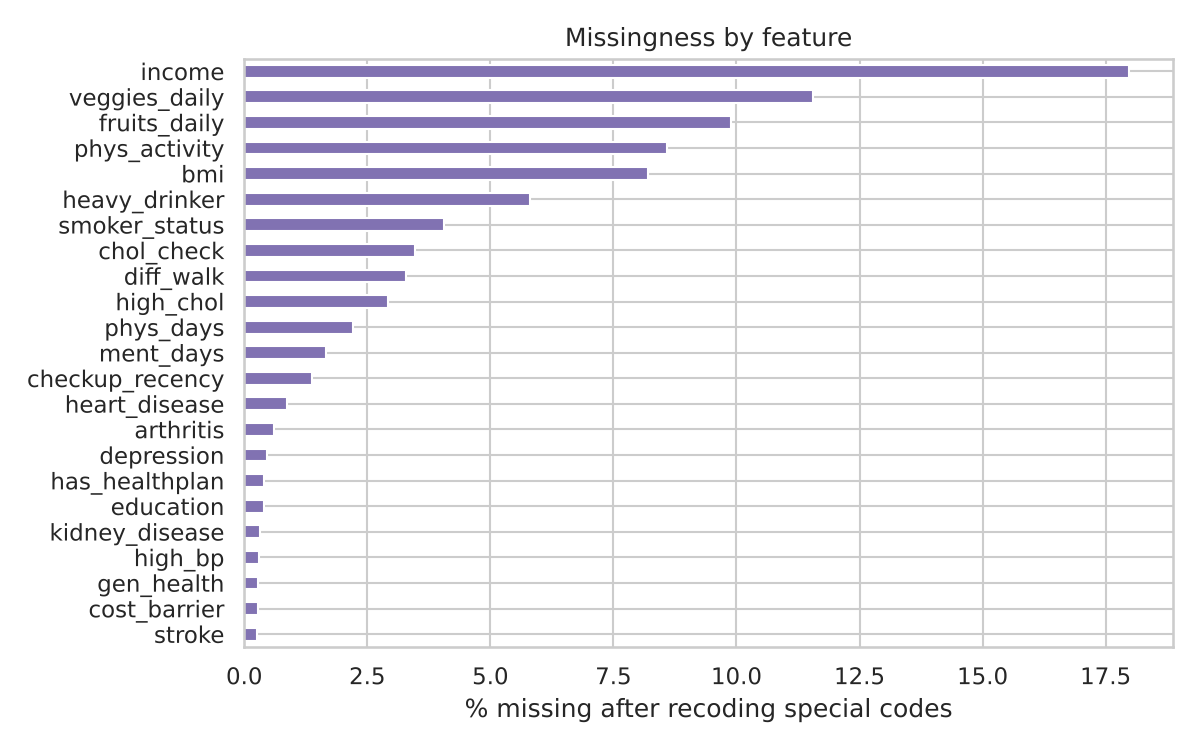
\includegraphics[width=0.48\linewidth]{fig02_missingness.png}
\caption{Left: class distribution, unweighted and survey-weighted. Right: percentage of missing values per feature after recoding special codes.}
\end{figure}

\begin{figure}[H]
\centering
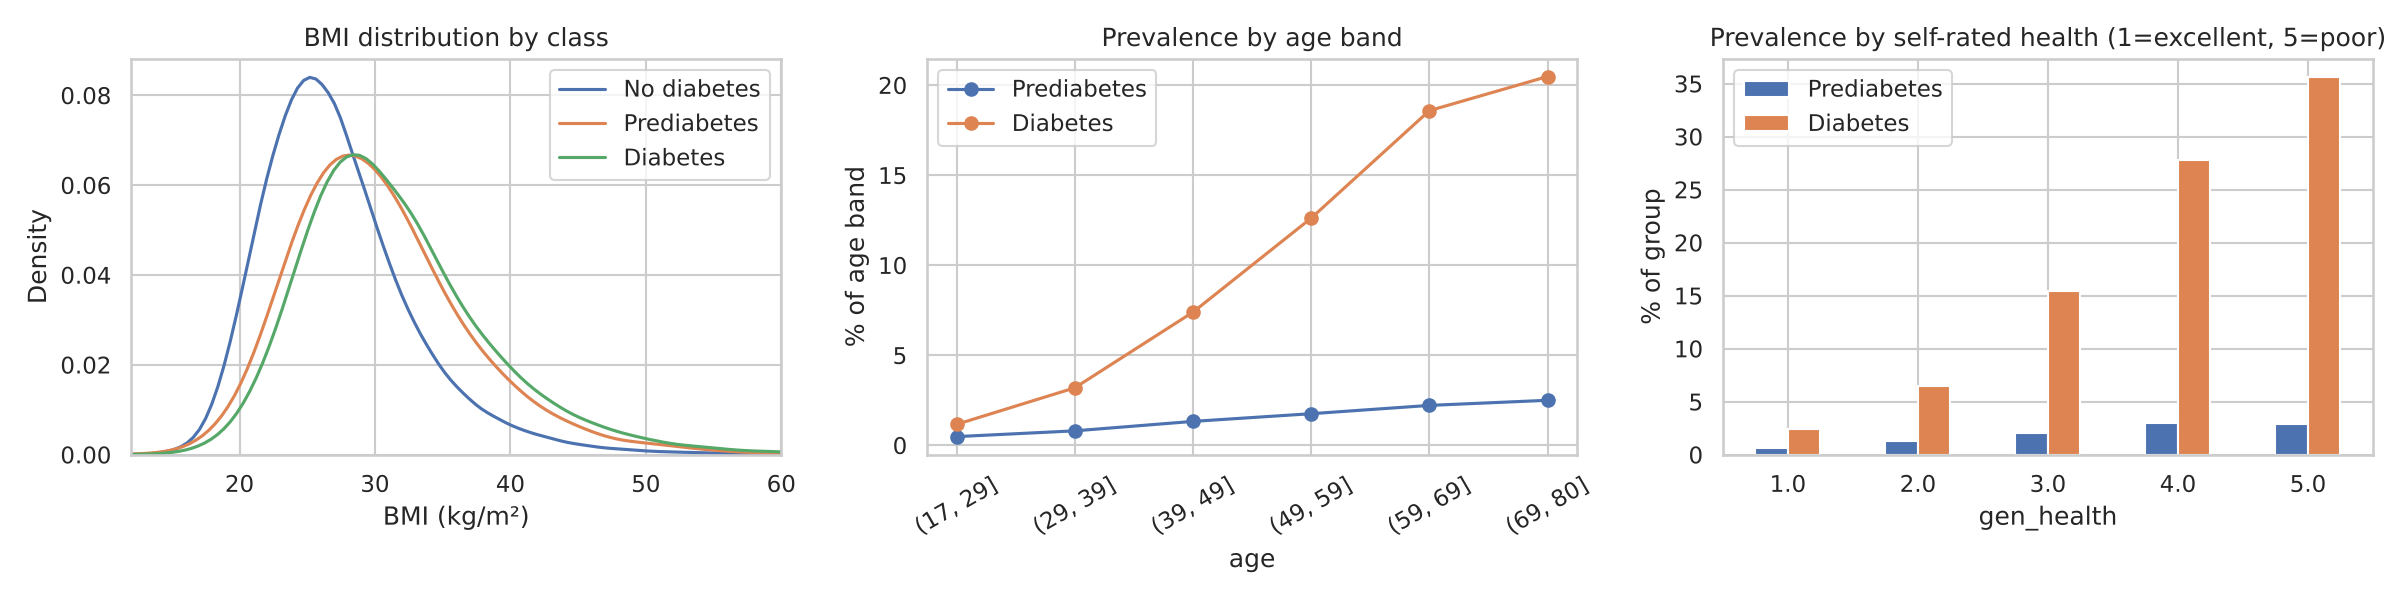
\includegraphics[width=\linewidth]{fig03_distributions.png}
\caption{BMI distribution by class, prevalence by age band, and prevalence by self-rated general health.}
\end{figure}

\begin{figure}[H]
\centering
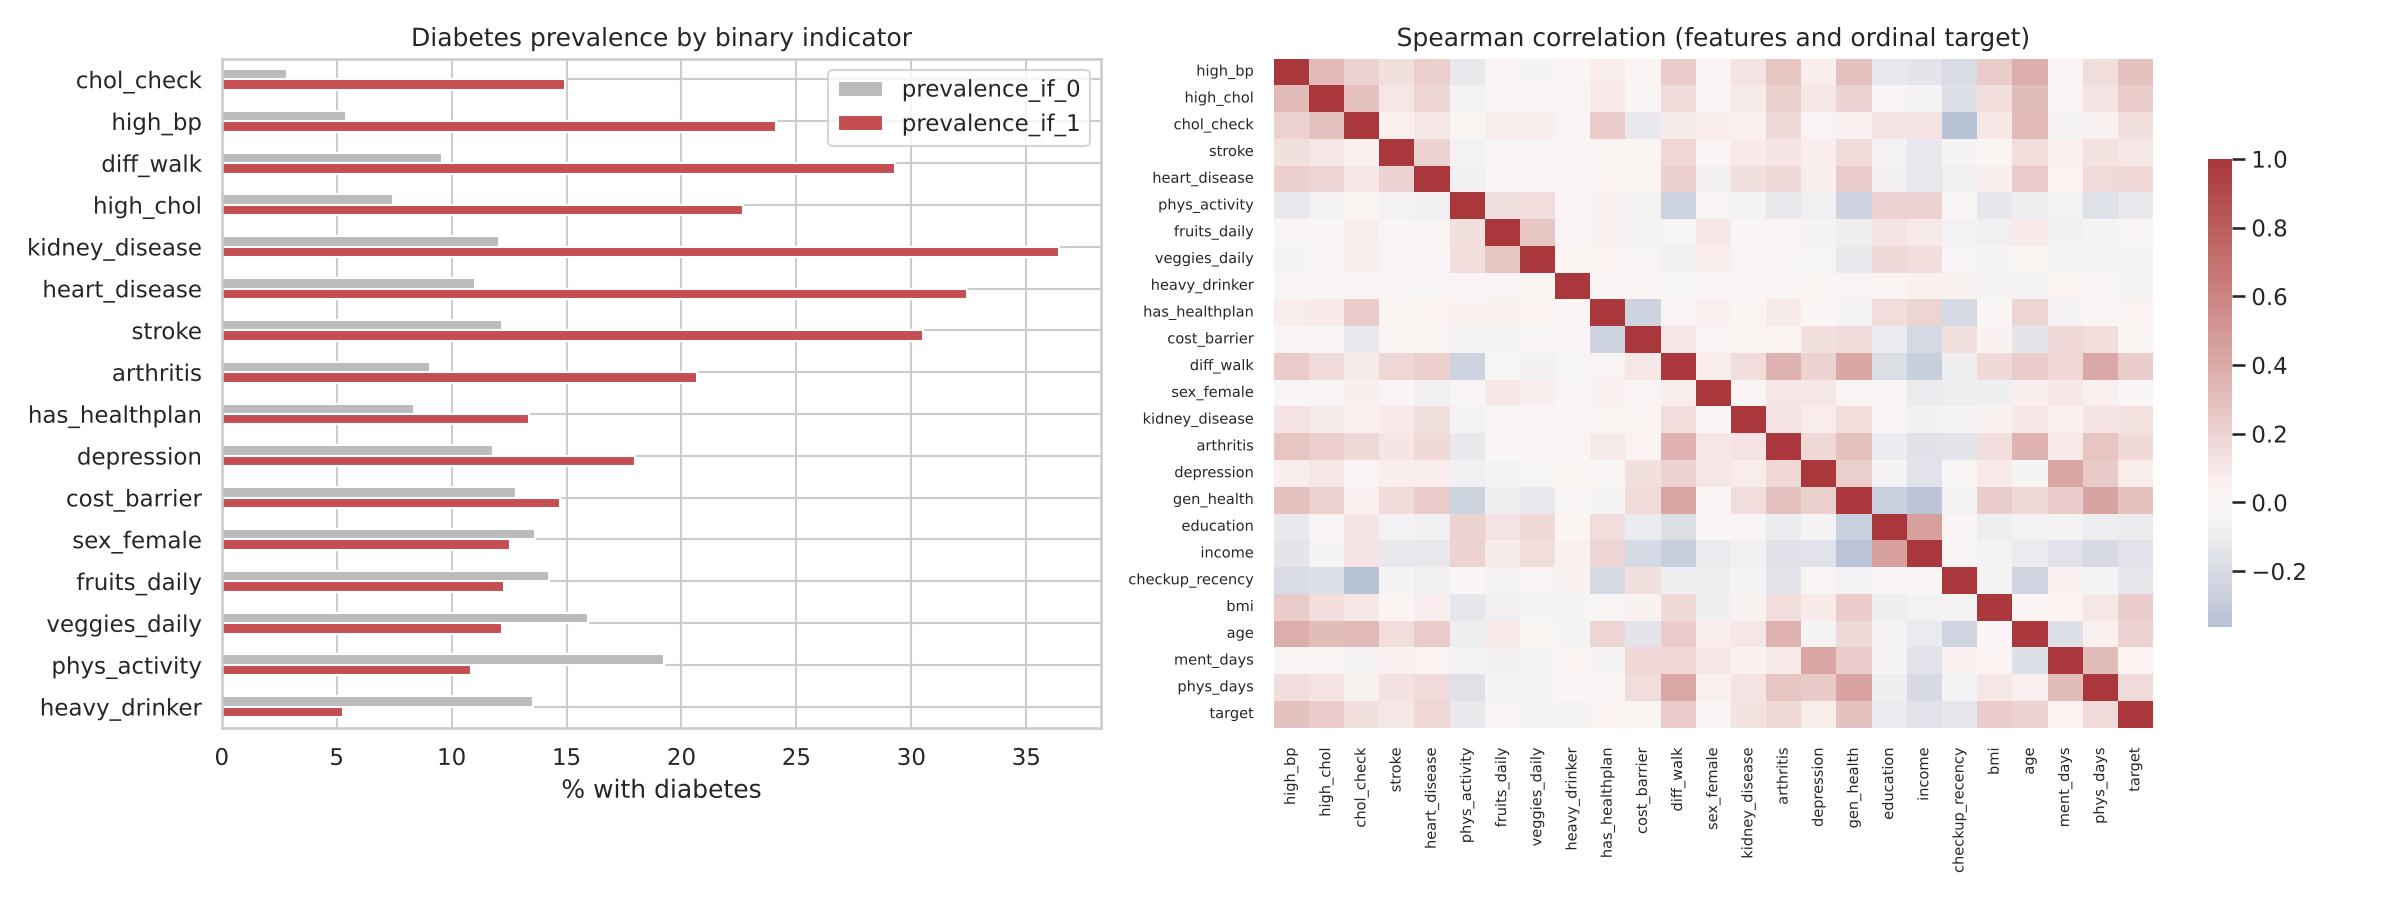
\includegraphics[width=\linewidth]{fig04_associations.png}
\caption{Diabetes prevalence by binary indicator (left) and Spearman correlations among features and the ordinal target (right).}
\end{figure}

\begin{figure}[H]
\centering
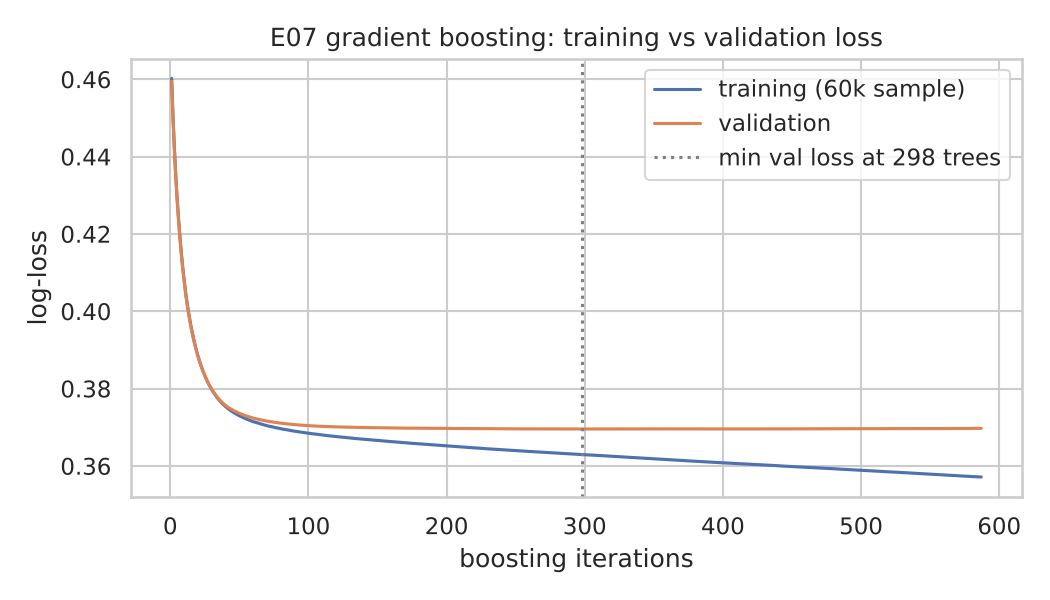
\includegraphics[width=0.48\linewidth]{fig06_boosting_learning_curve.png}\hfill
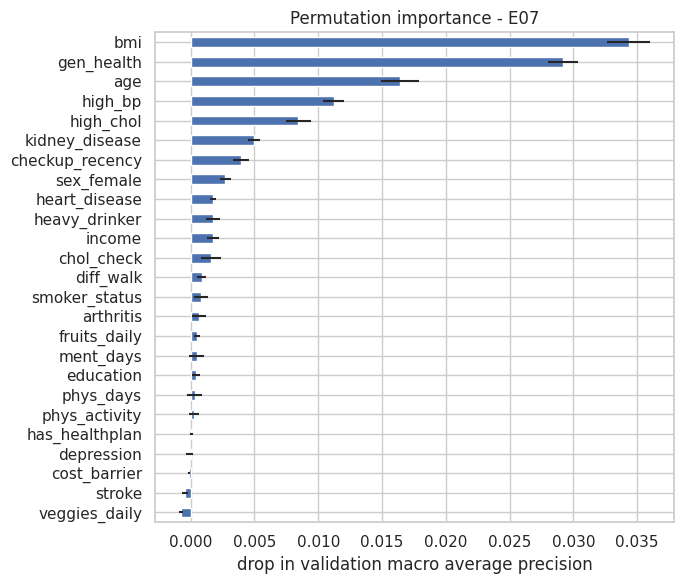
\includegraphics[width=0.48\linewidth]{fig10_permutation_importance.png}
\caption{Left: training vs.\ validation log-loss across boosting iterations for E07. Right: permutation importance (drop in validation macro AP) for E07.}
\end{figure}

\begin{figure}[H]
\centering
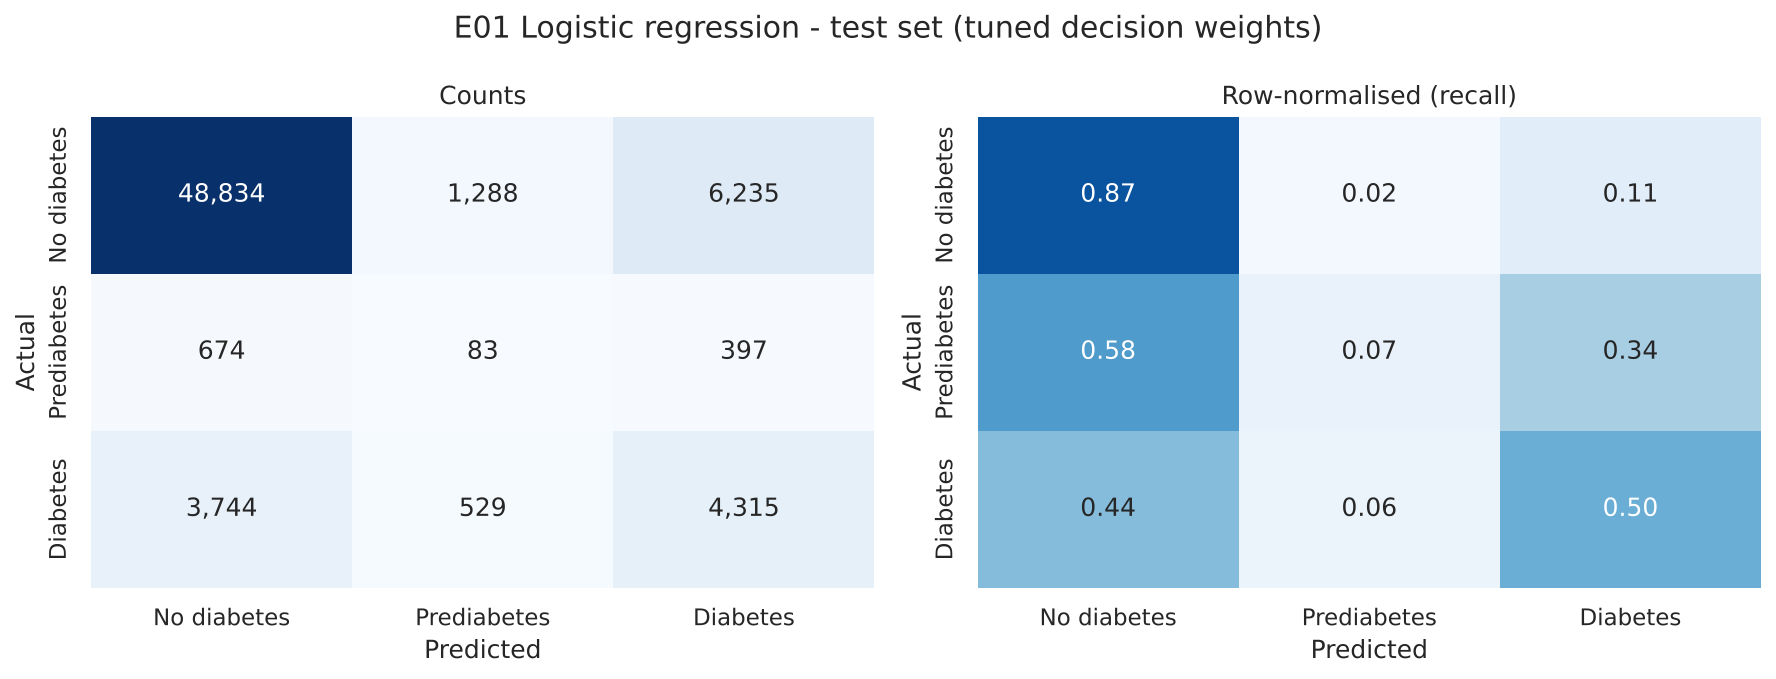
\includegraphics[width=0.49\linewidth]{fig08_confusion_E01.png}\hfill
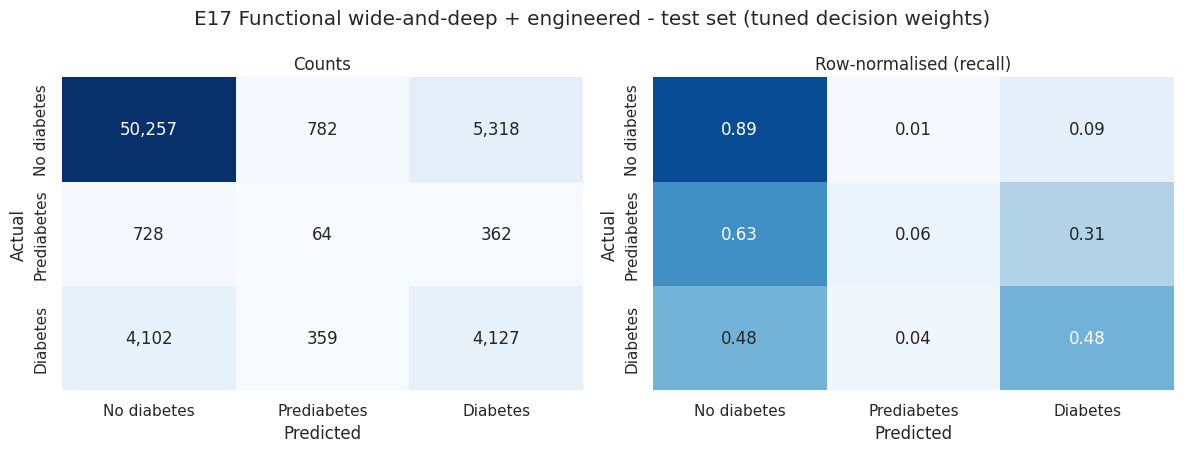
\includegraphics[width=0.49\linewidth]{fig08_confusion_E17.png}
\caption{Test-set confusion matrices for logistic regression (E01, left) and the wide-and-deep network (E17, right) with tuned decision weights.}
\end{figure}

\section{Reproducibility}
The environment (Python 3.13, scikit-learn 1.6.1, TensorFlow 2.21, Keras 3.13.2, SHAP 0.52.0) is pinned in \texttt{requirements.txt} and recorded in \texttt{reports/environment.json}. The SHA-256 of the data file used is \texttt{bfe9e629\ldots ad300b1b9}. Saved artifacts (full scikit-learn pipeline, Keras model with its preprocessor, and metadata containing decision weights and the screening threshold) were reloaded and reproduced the in-memory predictions exactly.
